\documentclass[]{article}
\usepackage{lmodern}
\usepackage{amssymb,amsmath}
\usepackage{ifxetex,ifluatex}
\usepackage{fixltx2e} % provides \textsubscript
\ifnum 0\ifxetex 1\fi\ifluatex 1\fi=0 % if pdftex
  \usepackage[T1]{fontenc}
  \usepackage[utf8]{inputenc}
\else % if luatex or xelatex
  \ifxetex
    \usepackage{mathspec}
  \else
    \usepackage{fontspec}
  \fi
  \defaultfontfeatures{Ligatures=TeX,Scale=MatchLowercase}
\fi
% use upquote if available, for straight quotes in verbatim environments
\IfFileExists{upquote.sty}{\usepackage{upquote}}{}
% use microtype if available
\IfFileExists{microtype.sty}{%
\usepackage{microtype}
\UseMicrotypeSet[protrusion]{basicmath} % disable protrusion for tt fonts
}{}
\usepackage[margin=1in]{geometry}
\usepackage{hyperref}
\hypersetup{unicode=true,
            pdftitle={Milestone 3},
            pdfauthor={Anh Le, Eve Wicksteed},
            pdfborder={0 0 0},
            breaklinks=true}
\urlstyle{same}  % don't use monospace font for urls
\usepackage{longtable,booktabs}
\usepackage{graphicx,grffile}
\makeatletter
\def\maxwidth{\ifdim\Gin@nat@width>\linewidth\linewidth\else\Gin@nat@width\fi}
\def\maxheight{\ifdim\Gin@nat@height>\textheight\textheight\else\Gin@nat@height\fi}
\makeatother
% Scale images if necessary, so that they will not overflow the page
% margins by default, and it is still possible to overwrite the defaults
% using explicit options in \includegraphics[width, height, ...]{}
\setkeys{Gin}{width=\maxwidth,height=\maxheight,keepaspectratio}
\IfFileExists{parskip.sty}{%
\usepackage{parskip}
}{% else
\setlength{\parindent}{0pt}
\setlength{\parskip}{6pt plus 2pt minus 1pt}
}
\setlength{\emergencystretch}{3em}  % prevent overfull lines
\providecommand{\tightlist}{%
  \setlength{\itemsep}{0pt}\setlength{\parskip}{0pt}}
\setcounter{secnumdepth}{0}
% Redefines (sub)paragraphs to behave more like sections
\ifx\paragraph\undefined\else
\let\oldparagraph\paragraph
\renewcommand{\paragraph}[1]{\oldparagraph{#1}\mbox{}}
\fi
\ifx\subparagraph\undefined\else
\let\oldsubparagraph\subparagraph
\renewcommand{\subparagraph}[1]{\oldsubparagraph{#1}\mbox{}}
\fi

%%% Use protect on footnotes to avoid problems with footnotes in titles
\let\rmarkdownfootnote\footnote%
\def\footnote{\protect\rmarkdownfootnote}

%%% Change title format to be more compact
\usepackage{titling}

% Create subtitle command for use in maketitle
\providecommand{\subtitle}[1]{
  \posttitle{
    \begin{center}\large#1\end{center}
    }
}

\setlength{\droptitle}{-2em}

  \title{Milestone 3}
    \pretitle{\vspace{\droptitle}\centering\huge}
  \posttitle{\par}
    \author{Anh Le, Eve Wicksteed}
    \preauthor{\centering\large\emph}
  \postauthor{\par}
    \date{}
    \predate{}\postdate{}
  

\begin{document}
\maketitle

\hypertarget{the-impact-of-weather-on-air-quality}{%
\section{The impact of weather on air
quality}\label{the-impact-of-weather-on-air-quality}}

\hypertarget{introduction}{%
\subsection{Introduction}\label{introduction}}

The adverse affects of air pollution on health are well documented and
air pollution can lead to a large range of diseases and increased
morbidity and mortality (Younger et al., 2008). Adverse health impacts
include, but are not limited to, lung cancer risk, respiritory
infections, allergic disease and asthma (Younger et al., 2008; Shea et
al., 2008). These health risks can affect a large proportion of the
population as many different groups are vulnerable to the effects of air
pollution including infants, children, the elderly, people with impaired
immune systems, and people who work or are physically active outdoors
(Matooane et al., 2004).

Because of the many, and severe, impacts of air quality, it is important
to understand patterns in the data. We have a dataset of air quality
observations as well as temperature and humidity data which we will use
to gain understanding of the patterns and impacts of weather on air
quality.

\hypertarget{research-question}{%
\subsection{Research question}\label{research-question}}

As stated above we would like to understand the impact of weather on air
quality. For this reason our research question is: - What is the affect
of temperature and humidity on the concentration of air pollutants, such
as benzene, titania, and tin oxide?

\hypertarget{data-and-methods}{%
\subsection{Data and methods}\label{data-and-methods}}

\hypertarget{data-description}{%
\subsubsection{Data Description}\label{data-description}}

The air quality
\href{https://archive.ics.uci.edu/ml/datasets/Air+Quality}{dataset} used
in this analysis was obtained from the University of California Irvine
Machine learning Repository. It was contributed by Saverio De Vito from
the National Agency for New Technologies, Energy and Sustainable
Economic Development.

The dataset contains 15 variables and 9358 observations of hourly
averaged responses from an Air Quality Chemical Multisensor Device. Data
were recorded from March 2004 to February 2005, in a significantly
polluted area, at road level, within a city in Italy. Variables include
the date and time each response was recorded, and the corresponding
concentrations of 13 air pollutants analyzed by the sensor device.
Missing values are tagged with -200 value. Below is the entire variable
set:

\begin{longtable}[]{@{}lll@{}}
\toprule
Variables & Type & Description\tabularnewline
\midrule
\endhead
Date & character & Date (DD/MM/YYYY)\tabularnewline
Time & time & Time (HH.MM.SS)\tabularnewline
CO(GT) & double & True hourly averaged concentration CO in mg/m\^{}3
(reference analyzer)\tabularnewline
PT08.S1(CO) & integer & PT08.S1 (tin oxide) hourly averaged sensor
response (nominally CO targeted)\tabularnewline
NMHC(GT) & integer & True hourly averaged overall Non Metanic
HydroCarbons concentration in microg/m\^{}3 (reference
analyzer)\tabularnewline
C6H6(GT) & double & True hourly averaged Benzene concentration in
microg/m\^{}3 (reference analyzer)\tabularnewline
PT08.S2(NMHC) & integer & PT08.S2 (titania) hourly averaged sensor
response (nominally NMHC targeted)\tabularnewline
NOx(GT) & integer & True hourly averaged NOx concentration in ppb
(reference analyzer)\tabularnewline
PT08.S3(NOx) & integer & PT08.S3 (tungsten oxide) hourly averaged sensor
response (nominally NOx targeted)\tabularnewline
NO2(GT) & integer & True hourly averaged NO2 concentration in
microg/m\^{}3 (reference analyzer)\tabularnewline
PT08.S4(NO2) & integer & PT08.S4 (tungsten oxide) hourly averaged sensor
response (nominally NO2 targeted)\tabularnewline
PT08.S5(O3) & integer & PT08.S5 (indium oxide) hourly averaged sensor
response (nominally O3 targeted)\tabularnewline
T & double & Temperature in °C\tabularnewline
RH & double & Relative Humidity (\%)\tabularnewline
AH & double & AH Absolute Humidity\tabularnewline
\bottomrule
\end{longtable}

Here you can see the data that we use:

\begin{verbatim}
## Warning in rbind(names(probs), probs_f): number of columns of result is not
## a multiple of vector length (arg 1)
\end{verbatim}

\begin{verbatim}
## Warning: 7 parsing failures.
## row # A tibble: 5 x 5 col     row col         expected       actual file                              expected   <int> <chr>       <chr>          <chr>  <chr>                             actual 1  1132 Tungsten_o~ no trailing c~ e3     '/Users/lenguyetanh/Documents/Gi~ file 2  2179 Tungsten_o~ no trailing c~ e3     '/Users/lenguyetanh/Documents/Gi~ row 3  3570 Tungsten_o~ no trailing c~ e3     '/Users/lenguyetanh/Documents/Gi~ col 4  6331 NOx         no trailing c~ e3     '/Users/lenguyetanh/Documents/Gi~ expected 5  7594 Tungsten_o~ no trailing c~ e3     '/Users/lenguyetanh/Documents/Gi~
## ... ................. ... ........................................................................... ........ ........................................................................... ...... ........................................................................... .... ........................................................................... ... ........................................................................... ... ........................................................................... ........ ...........................................................................
## See problems(...) for more details.
\end{verbatim}

\includegraphics{milestone3_files/figure-latex/read data-1.pdf}

\hypertarget{methods}{%
\subsubsection{Methods}\label{methods}}

We are interested in the hourly averaged concentrations of air
pollutants, temperature and humidity. We ignore variables which have too
many missing data to increase the precision of this analysis. The air
pollutants that we will focus on are benzene, titania and tin oxide.
After dealing with the missing data, we will perform a linear regression
analysis using the OLS (ordinary least squares) method. Coefficients of
relevant variables will be plotted with confidence intervals.

\hypertarget{results}{%
\subsection{Results}\label{results}}

We first performed some exploratory data analysis of the air quality
data.

\hypertarget{exploratory-data-analysis}{%
\subsubsection{Exploratory data
analysis}\label{exploratory-data-analysis}}

\hypertarget{graph-1-correlogram-of-pollutants}{%
\paragraph{Graph 1: Correlogram of
pollutants}\label{graph-1-correlogram-of-pollutants}}

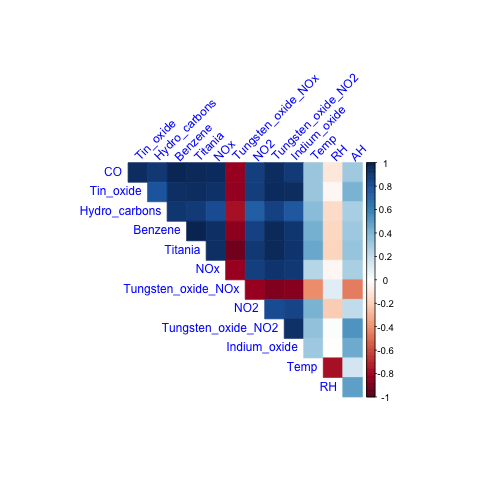
\includegraphics{../Images/correlation.png}

Looking at the correlations of the pollutants with weather, we can see
that for all pollutants except NOx, temperature (T) is positively
correlated, although weakly so. This means that higher temperatures
correspond to higher concentrations of the gases. Relative humidity (RH)
is negatively and correlated to temperature and has a weak negative
correlation to the concentrations of pollutants, except NOx. Absolute
humidity (AH) has stronger correlations, mostly positive, although, like
temperature, it has a negative correlation with NOx.

\hypertarget{graph-2-concentration-of-some-air-pollutants-temperature-humidity-over-time-daily-average}{%
\paragraph{Graph 2: Concentration of some Air Pollutants, Temperature,
Humidity over Time, daily
average}\label{graph-2-concentration-of-some-air-pollutants-temperature-humidity-over-time-daily-average}}

The plot below shows the \textbf{daily} averaged concentrations of some
of the pollutants (tin oxide, benzene, and Titania) for a year.

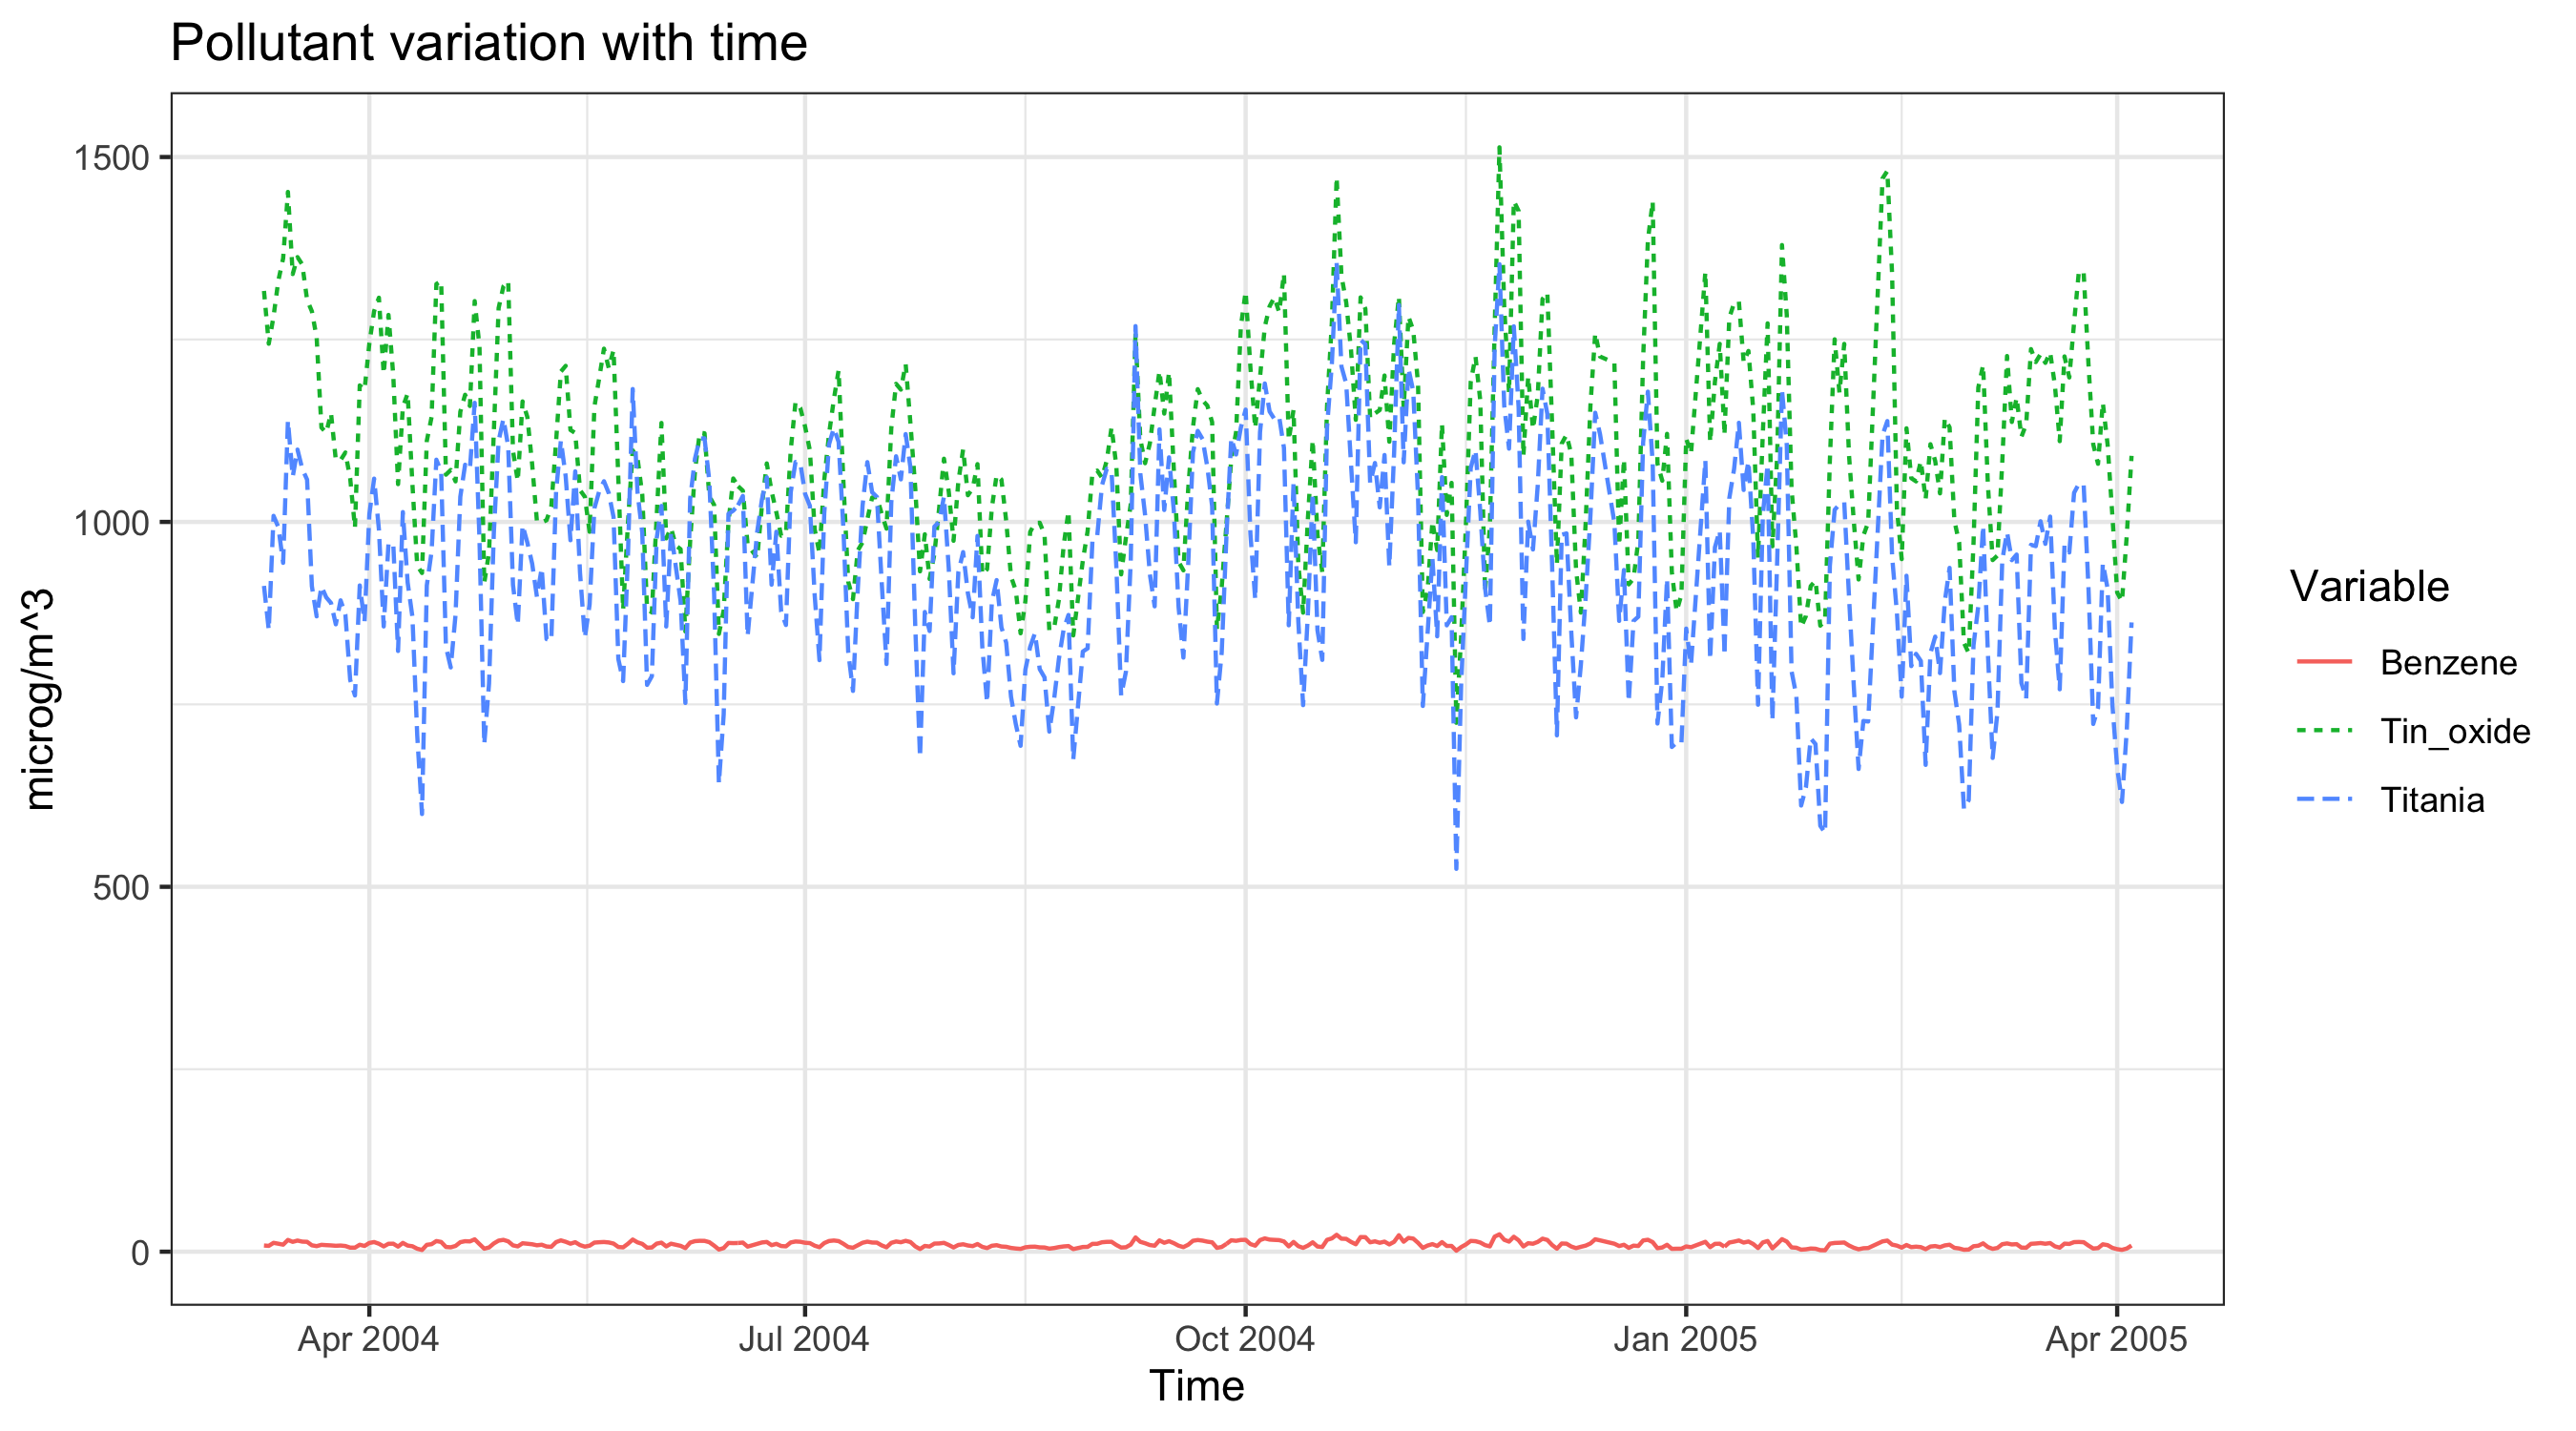
\includegraphics{../Images/pollutantsvstime.png}

\hypertarget{graph-3-concentration-temperature-and-humidity-over-time}{%
\paragraph{Graph 3: Concentration Temperature and Humidity over
Time}\label{graph-3-concentration-temperature-and-humidity-over-time}}

The plot below show the \textbf{daily} averaged values of temperature
and humidity for a year.

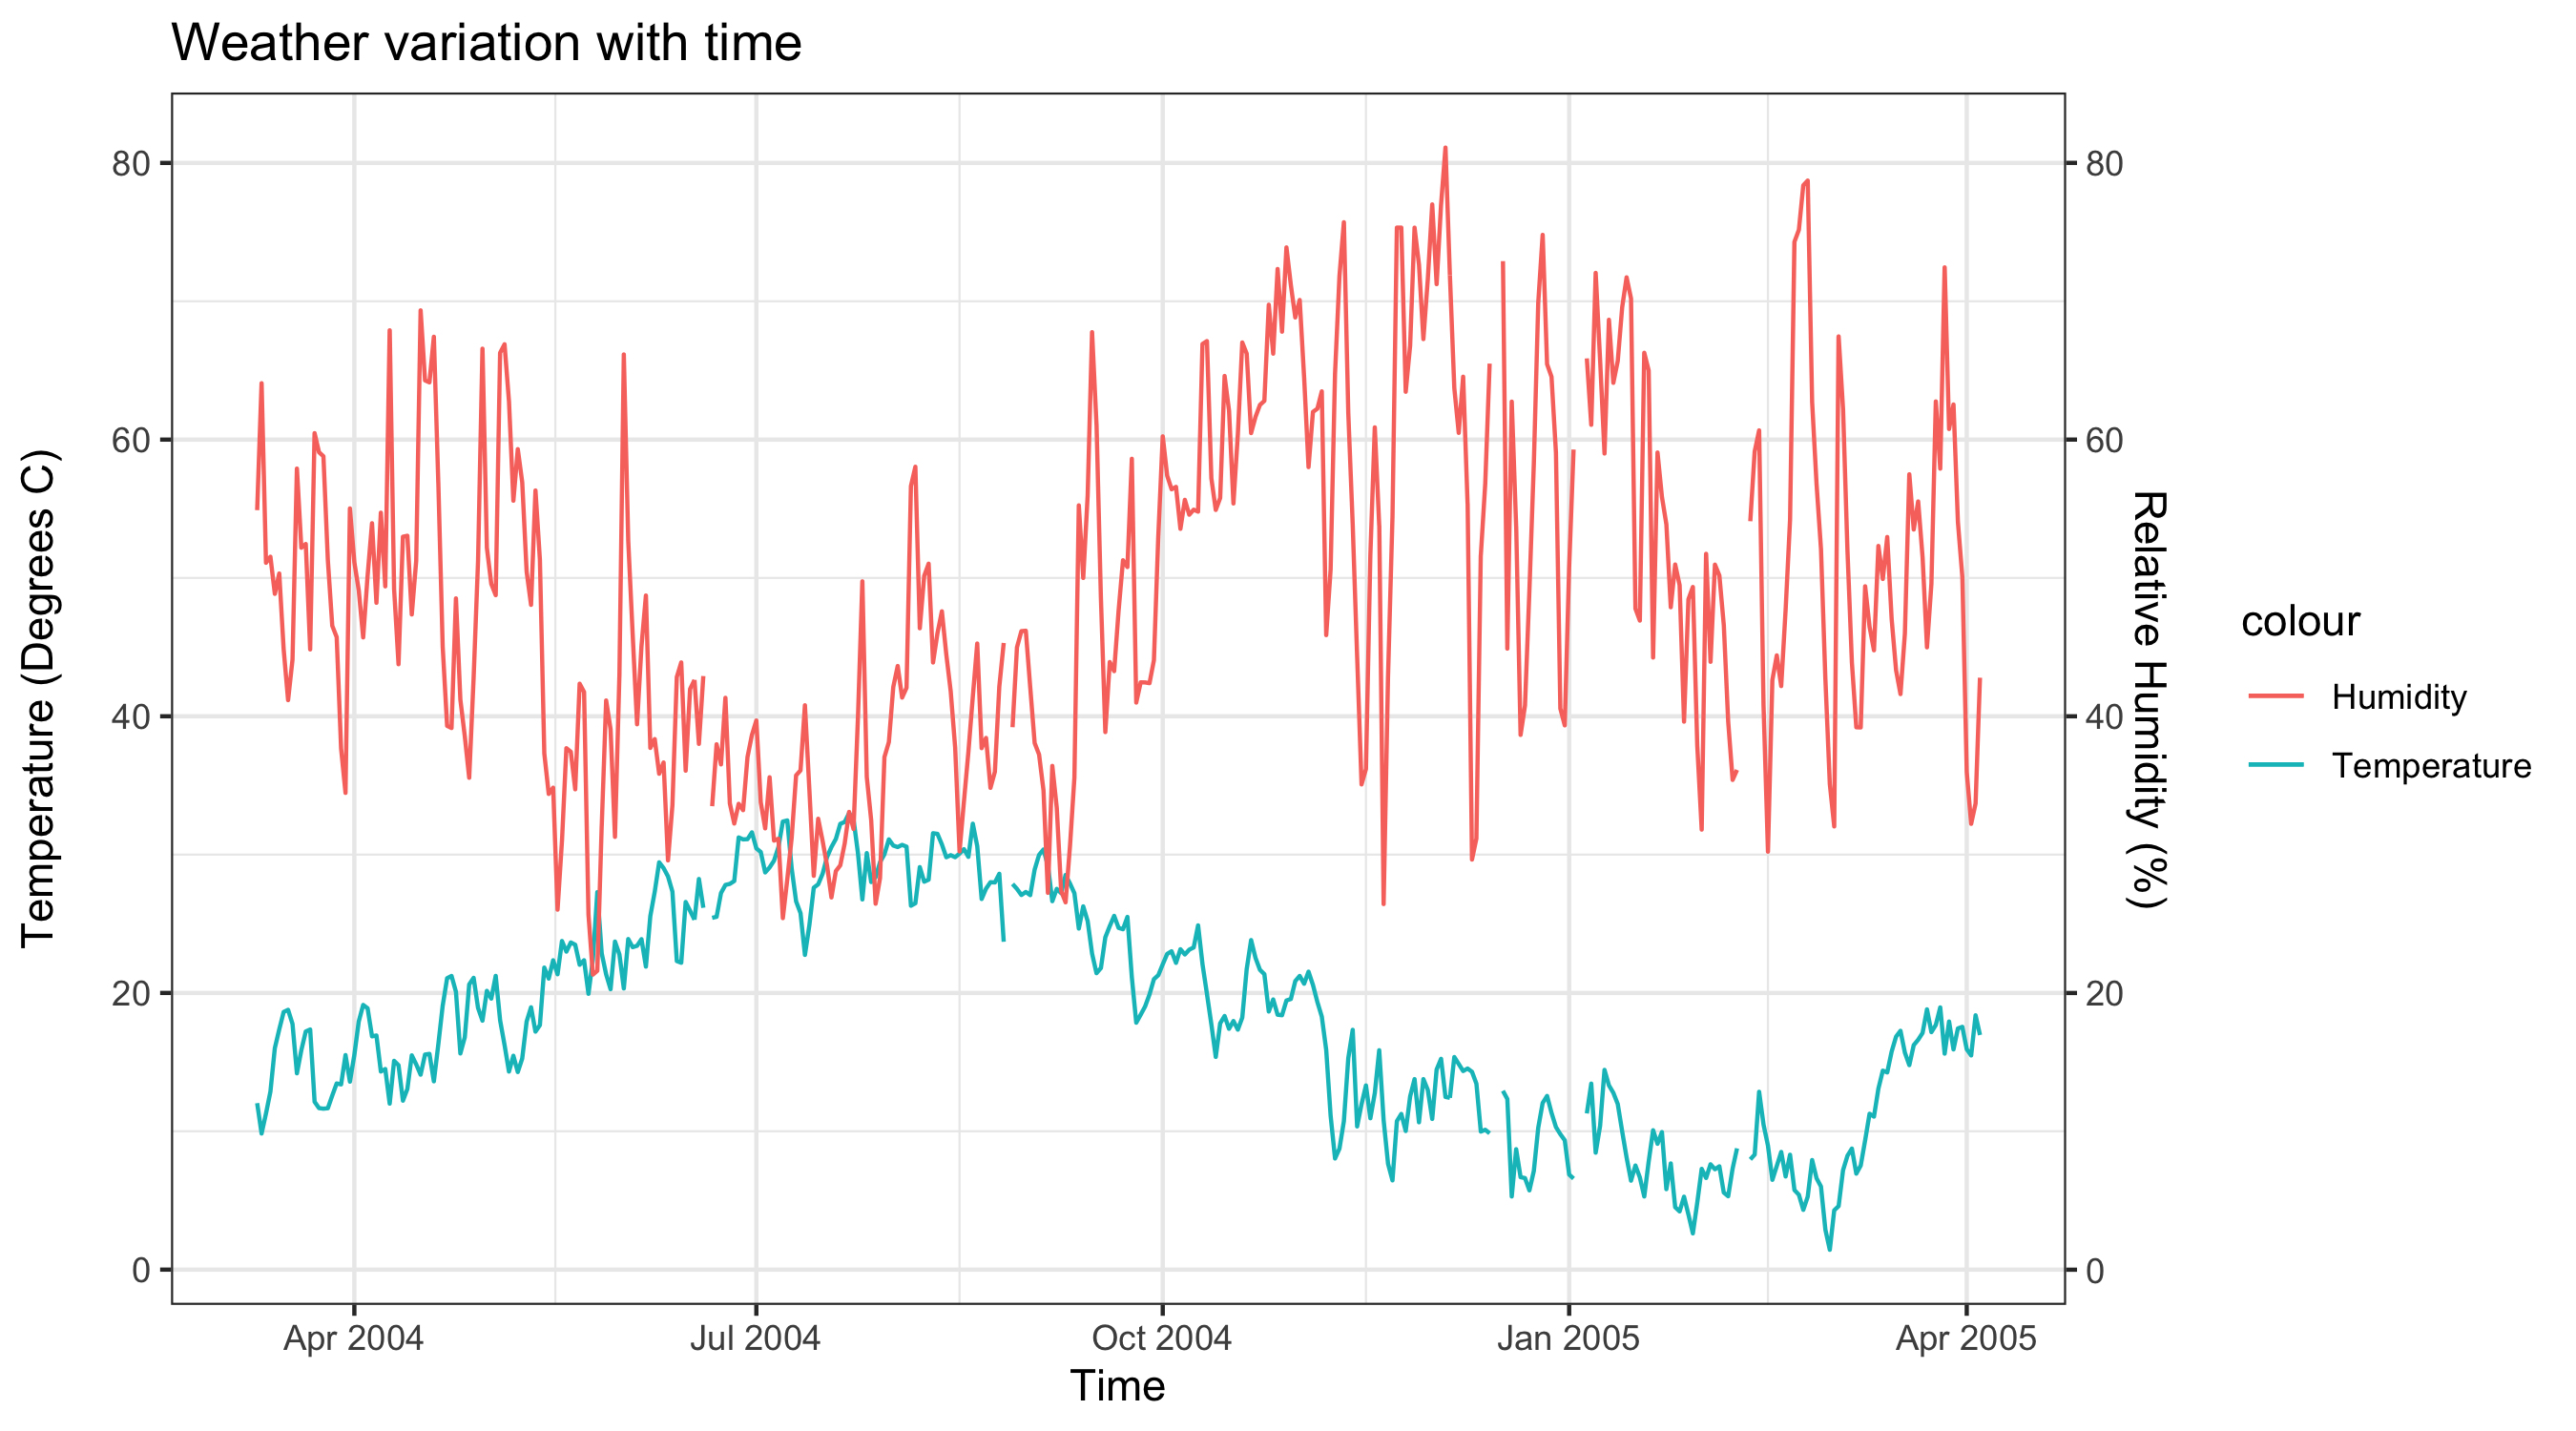
\includegraphics{../Images/weathervstime.png}

\hypertarget{graph-4-temperature-vs.benzene-concentration}{%
\paragraph{Graph 4: Temperature vs.~Benzene
concentration}\label{graph-4-temperature-vs.benzene-concentration}}

The following graph shows the relationship of benzene to temperature
over the year in which data was recorded. The plot suggests there is
perhaps a slight relationship. Linear regression in future work will
help to clarify the relationships between weather and pollutant
concentrations.

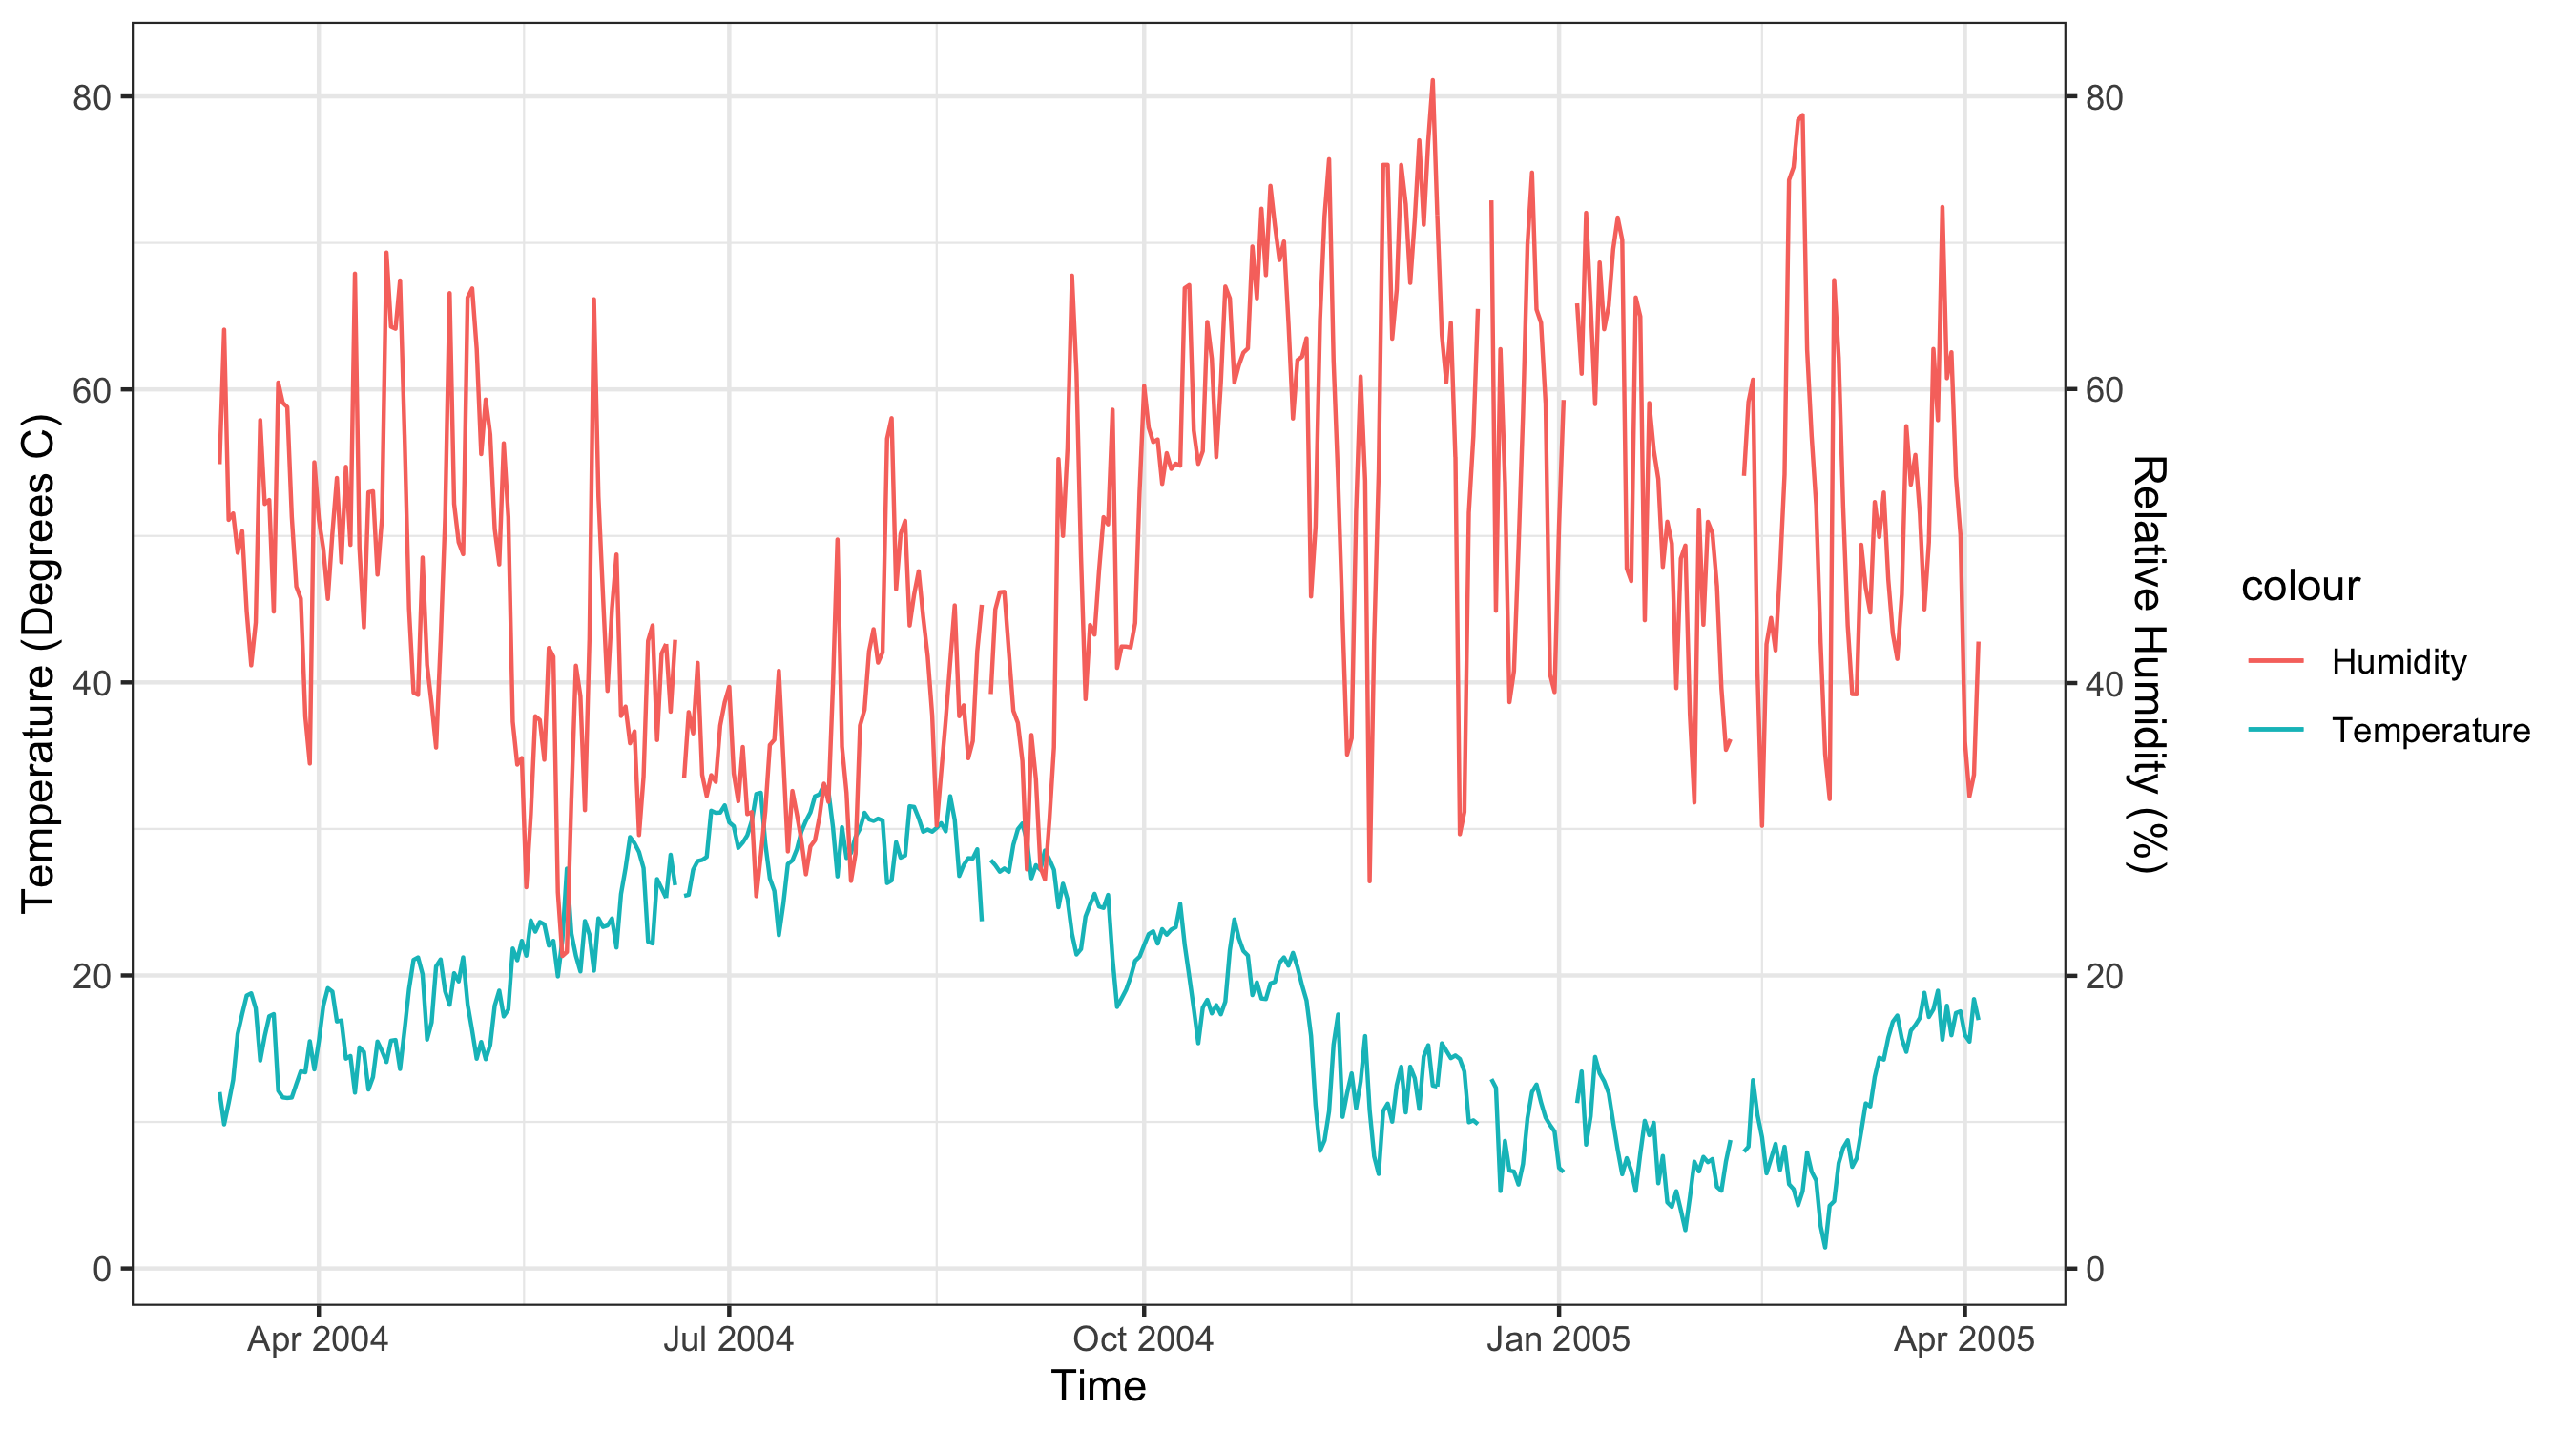
\includegraphics{../Images/tempvsbenzene.png}

\hypertarget{linear-regression}{%
\subsubsection{Linear regression}\label{linear-regression}}

We then perform linear regression of all the separate pollutants with
temperature and absolute humidity. The graph below shows the
coeffecients for linear regression for temperature and humidity with all
the various pollutants.

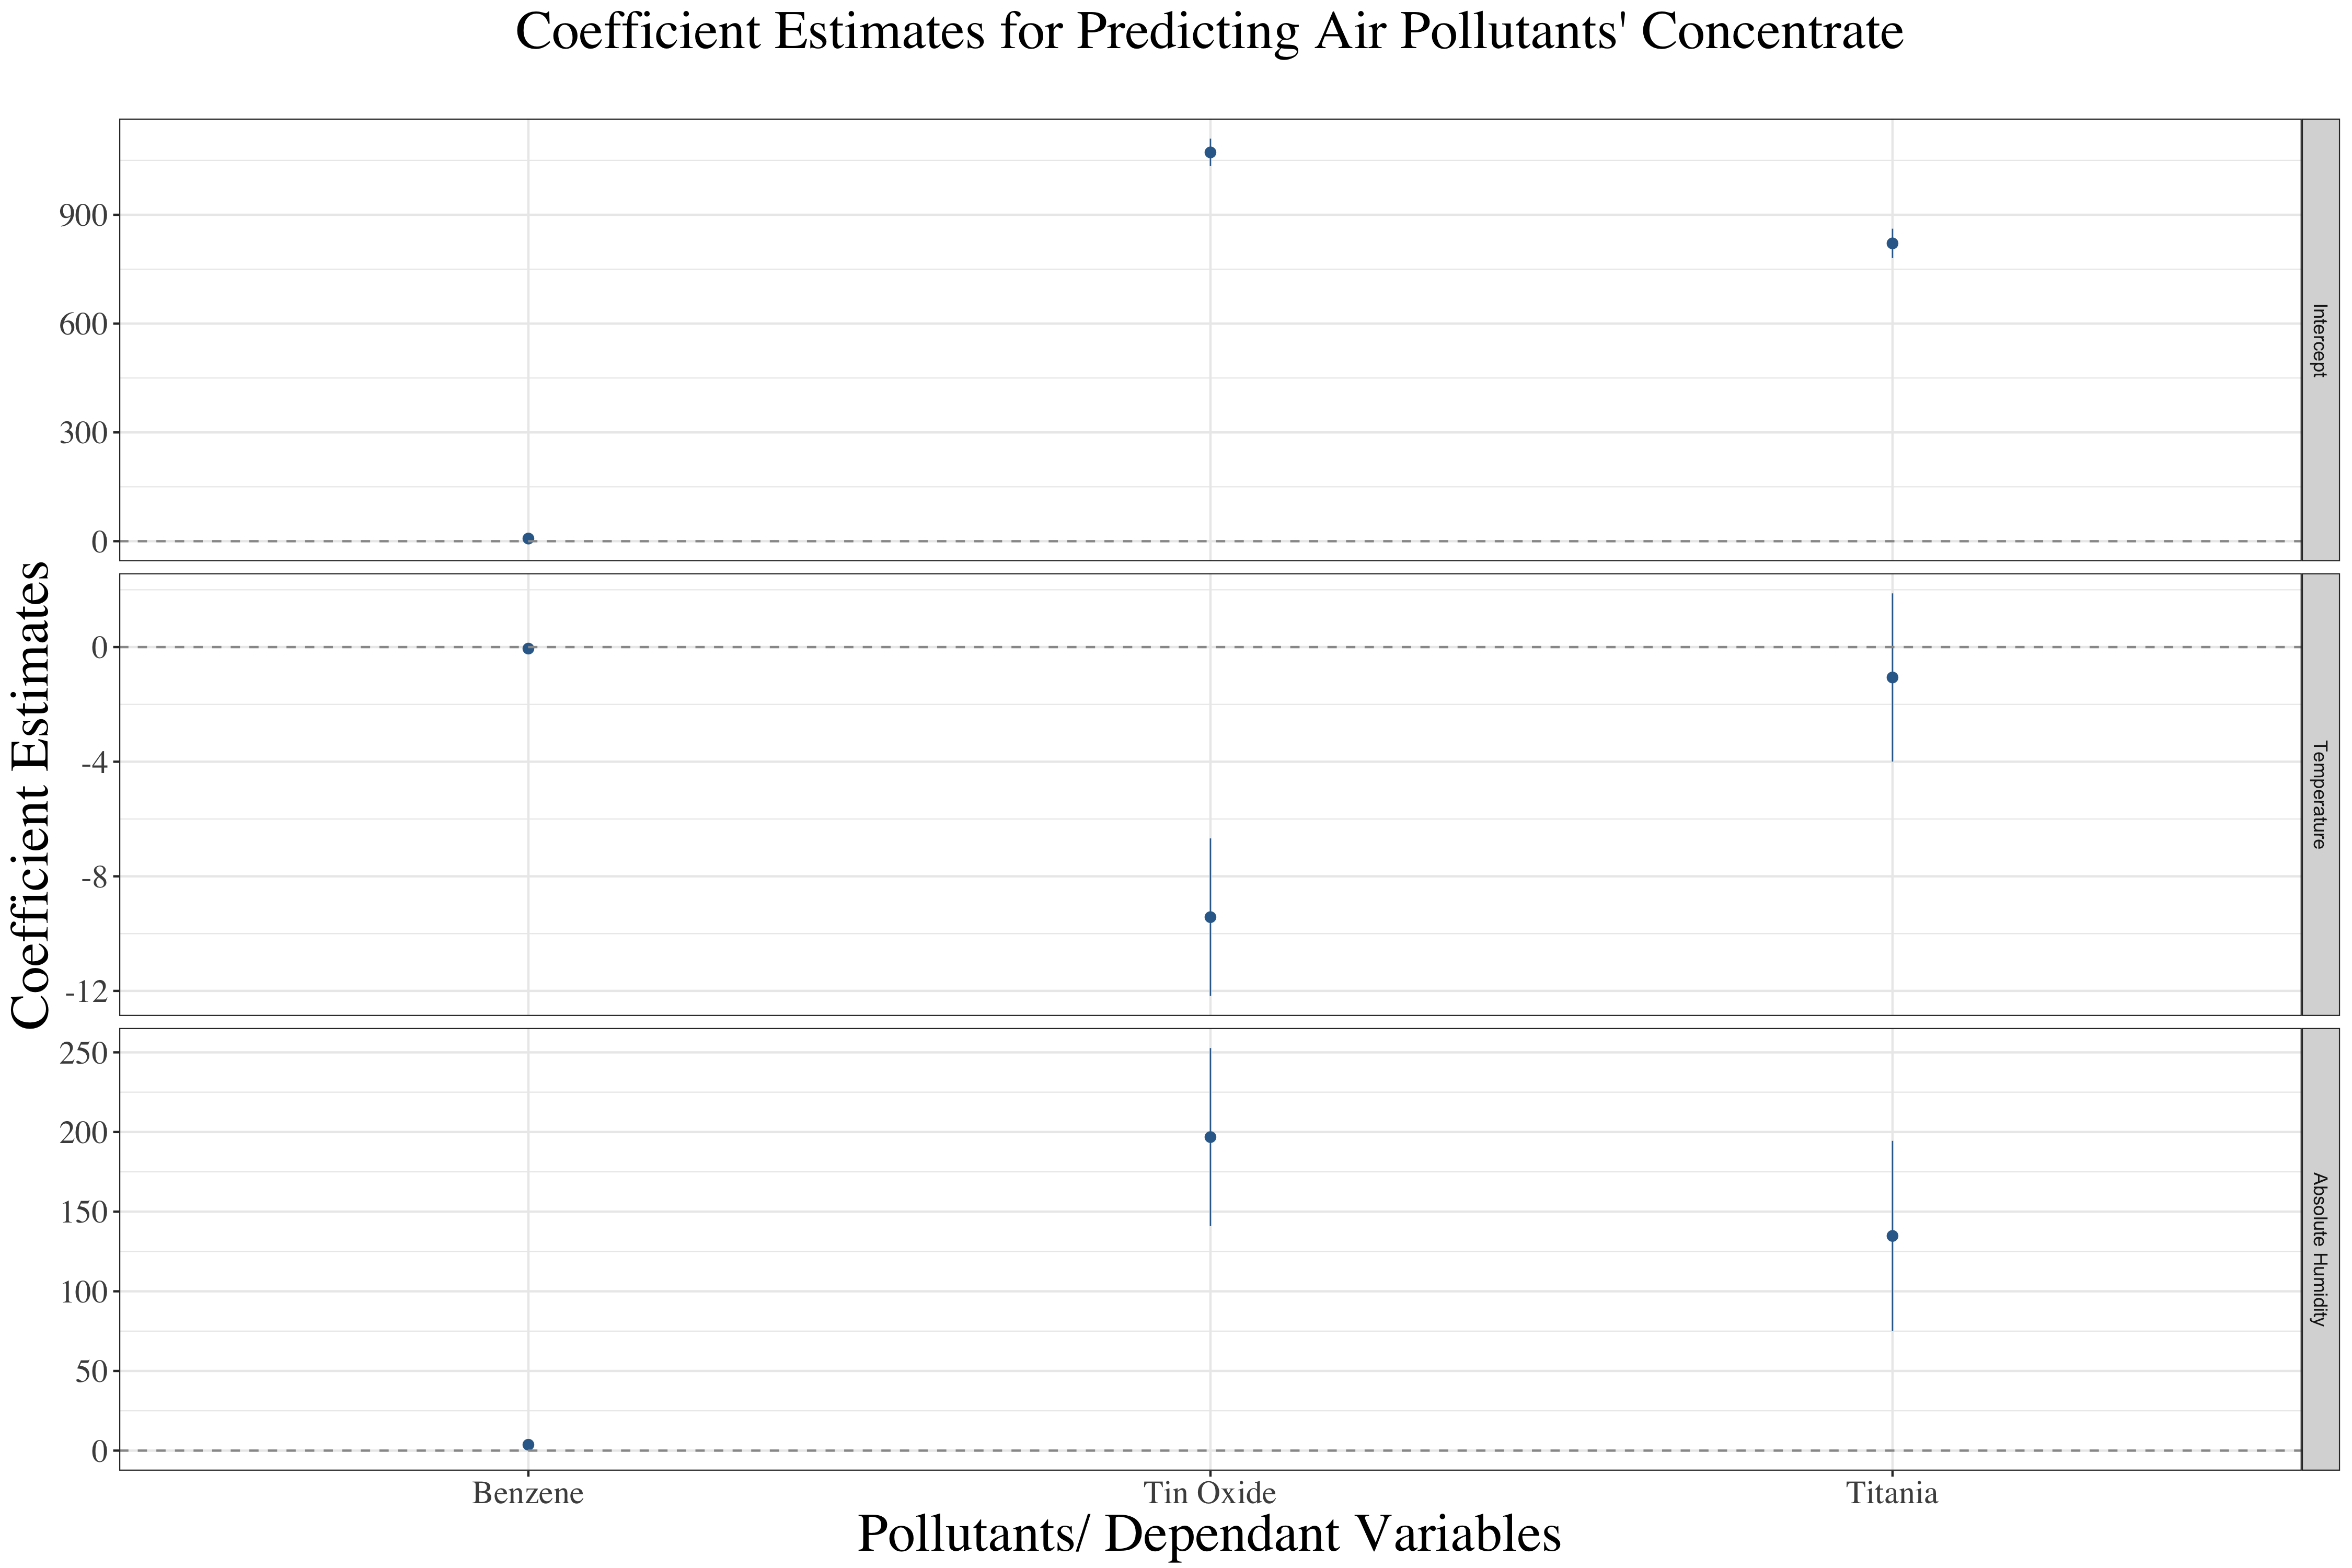
\includegraphics{../Images/CoefPlot_Group4.png} The table below shows an
example of the output of the linear regression model.

\begin{verbatim}
## # A tibble: 3 x 5
##   term        estimate std.error statistic  p.value
##   <chr>          <dbl>     <dbl>     <dbl>    <dbl>
## 1 (Intercept)   7.27      0.576      12.6  9.40e-31
## 2 Temp         -0.0523    0.0418     -1.25 2.12e- 1
## 3 AH            3.69      0.850       4.34 1.83e- 5
\end{verbatim}

The next plot shows three of the pollutants (Benzene, Titania and Tin
Oxide) plotted with temperature with the linear regression line also
plotted. From looking at the plots we can tell the the linear regression
line does not represent a lot of the data well. This is shown in the low
correlations values (in the plot titles).

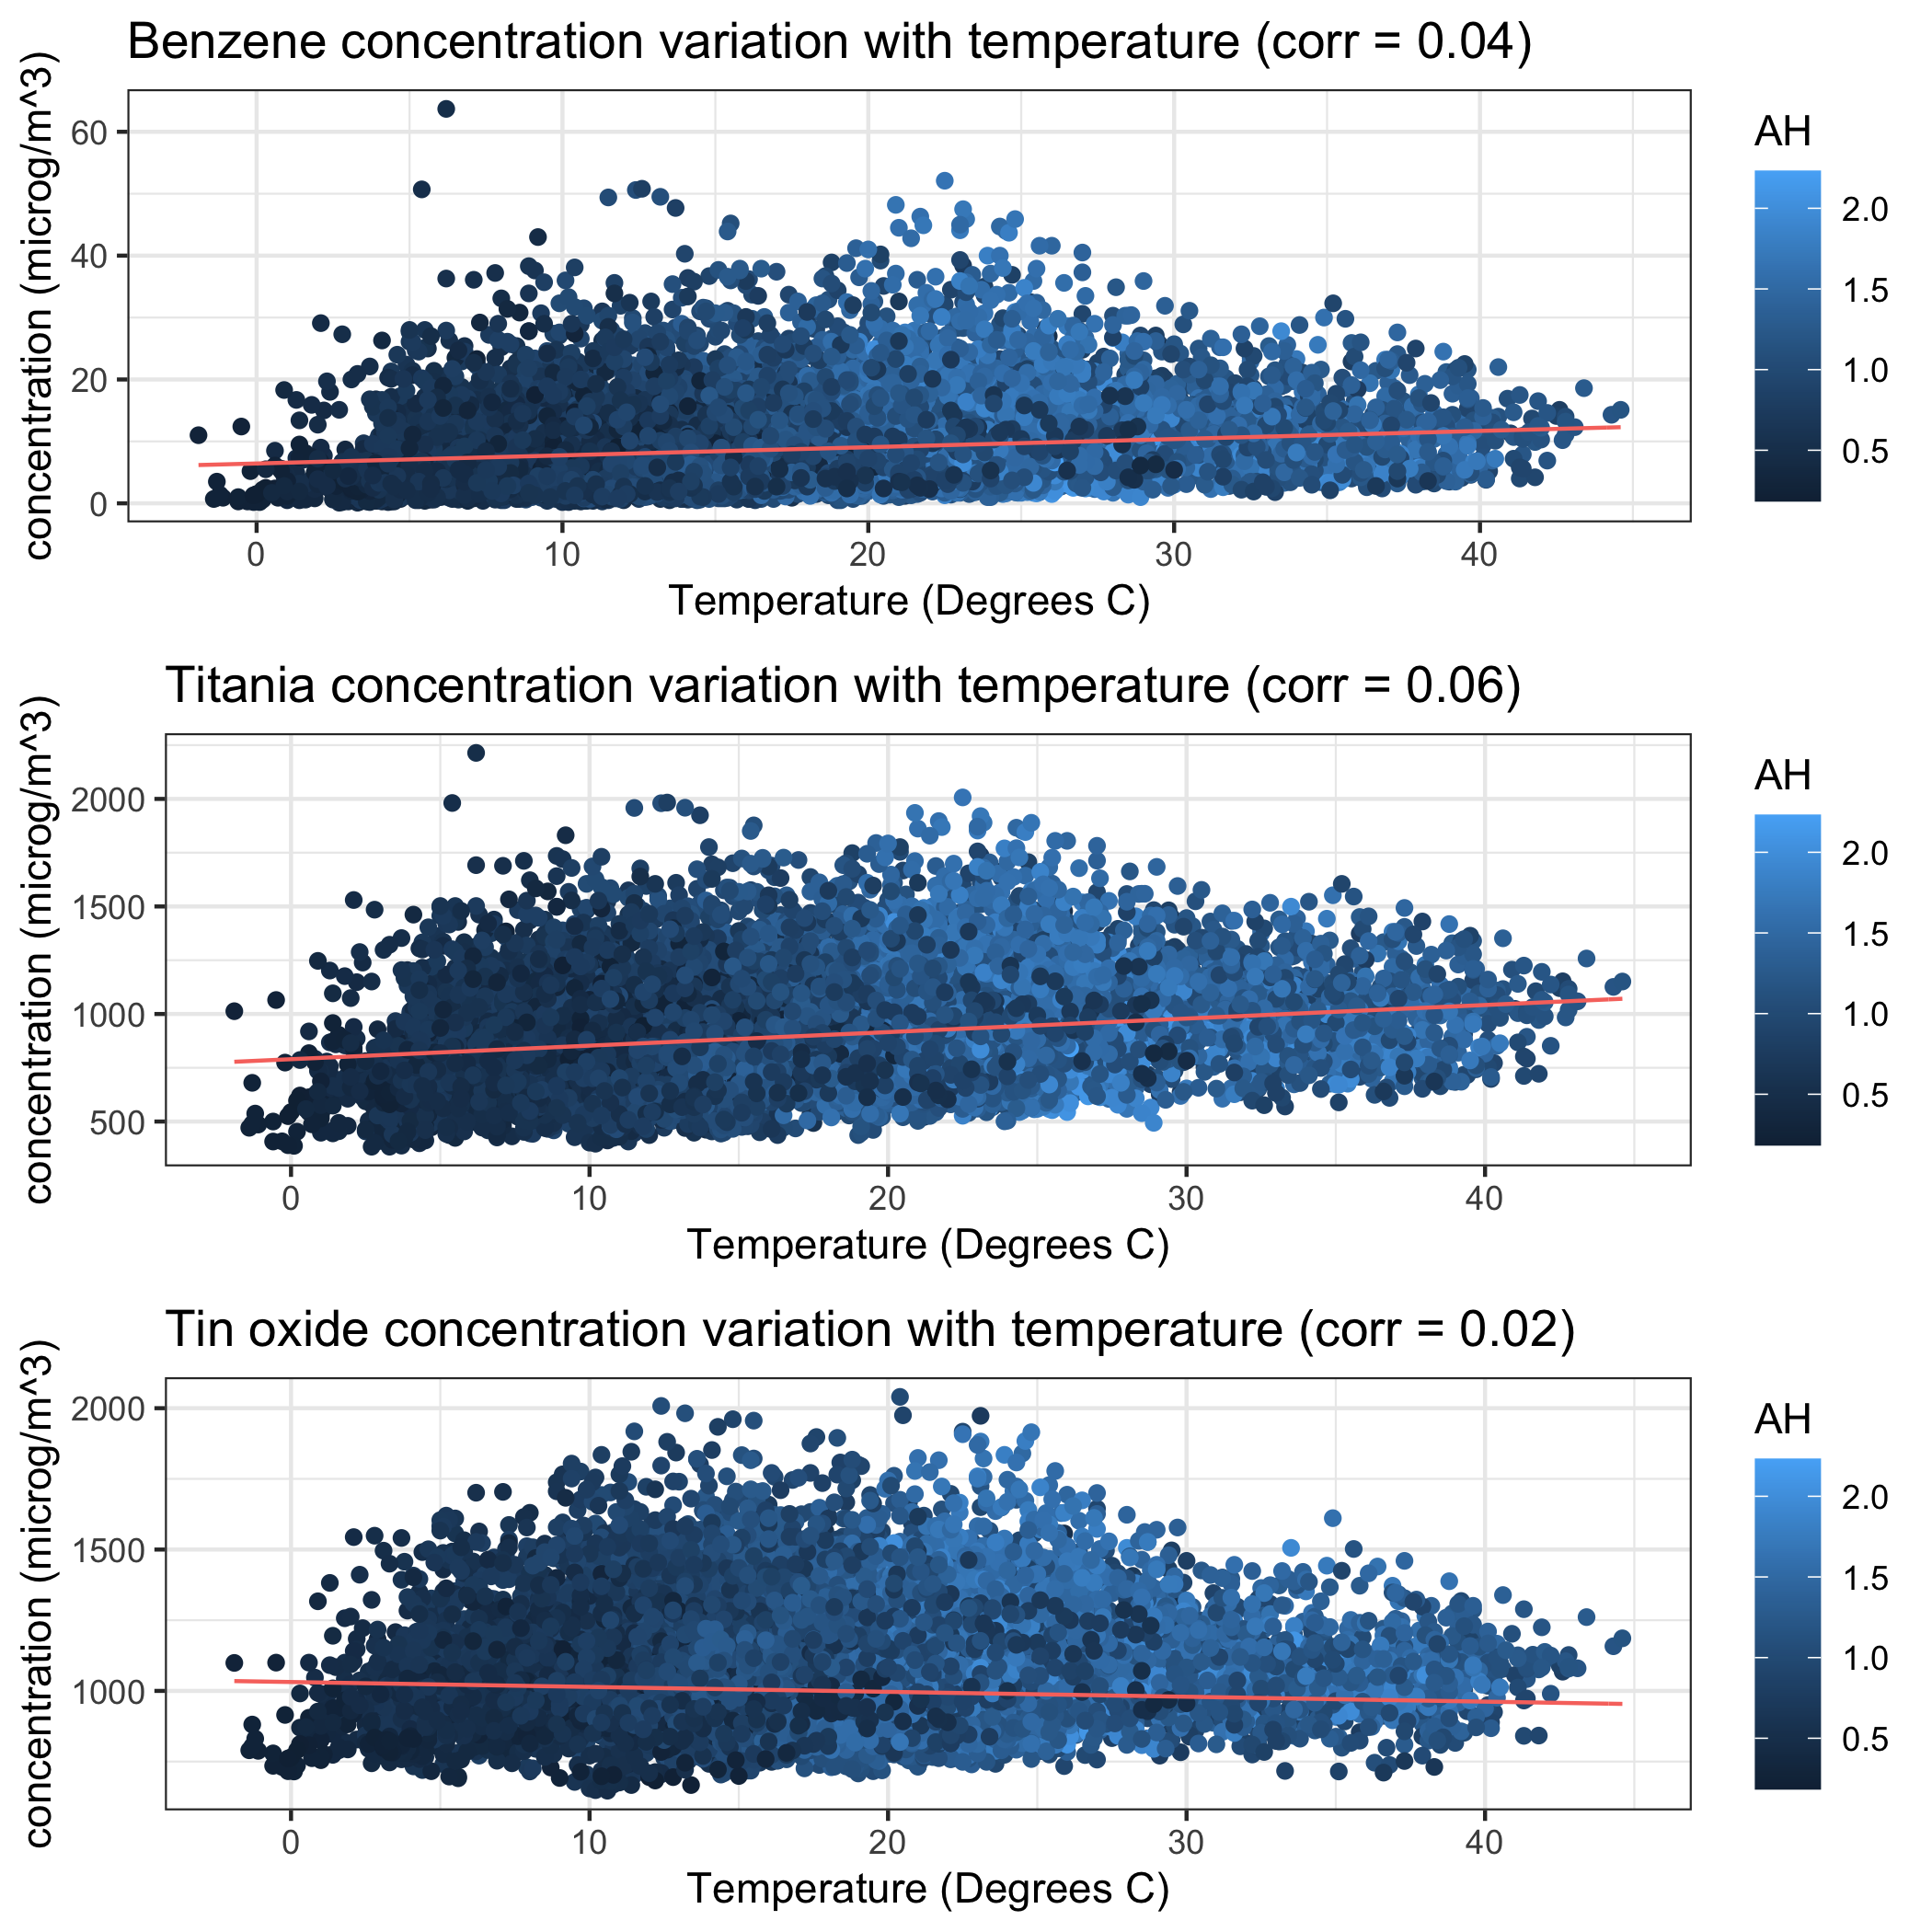
\includegraphics{../Images/more_lr_plots.png}

\hypertarget{discussion-and-conclusion}{%
\subsection{Discussion and Conclusion}\label{discussion-and-conclusion}}

It is clear that just looking at the values of temperature and humidity
on their own do not provide sufficient information to explain or predict
the given concentrations of pollutants. This can be seen in the figures
produced above where the linear regression line does not capture well
the variation of pollutants. Altough weather will affect some
pollutants, a more important determinant of pollutant concentrations is
emissions. These often vary with time of day and human activity and thus
a model incorporating weather as well as these other important variables
would likely be more accurate.

\hypertarget{references}{%
\subsection{References}\label{references}}

S. De Vito, E. Massera, M. Piga, L. Martinotto, G. Di Francia, On field
calibration of an electronic nose for benzene estimation in an urban
pollution monitoring scenario, Sensors and Actuators B: Chemical, Volume
129, Issue 2, 22 February 2008, Pages 750-757, ISSN 0925-4005.

Matooane, M., John, J., Oosthuizen, R., and Binedell, M. 2004.
Vulnerability of South African communities to air pollution. In: 8th
World Congress on Environmental Health. Durban, South Africa: Document
Transformation Technologies.

Shea, K., Truckner, R., Weber, R., and Peden, D. 2008. Climate change
and allergic disease. Journal of Allergy and Clinical Immunology,
122(3): 443-453.

Younger, M., Morrow-Almeida, H., Vindigni, S., and Dannenberg, A. 2008.
The Built Environment, Climate Change, and Health Opportunities for
Co-Benefits. American Journal of Preventative Medicine, 35 (5): 517-526.


\end{document}
